\documentclass[12pt]{article}

\usepackage{amsmath}
\usepackage{amsthm}
\usepackage[margin=1in]{geometry}
\usepackage{mathtools}
\usepackage{tikz}
\usetikzlibrary{arrows,automata}

\title{EECS 477 HW3}
\author{Andrew Mason}

\begin{document}
\maketitle

\begin{enumerate}
  % #1
  \item
  % #2
  \item
  % #3
  \item
  The MCNF problem in number 1 can be formulated as the following linear program:\\
  \begin{equation}
    \begin{split}
      \text{min}\ &4x_{ab}+6x_{ac}-2x_{bc}+5x_{be}-3x_{cd}+2x_{ed}\\
      \text{s.t.}\ &x_{ab}+x_{ac}=20\\
      &-x_{ab}+x_{bc}+x_{be}=5\\
      &-x_{ac}-x_{bc}+x_{cd}=-15\\
      &-x_{cd}-x_{ed}=-10\\
      &-x_{be}+x_{ed}=0\\
      &x_{ab}\geq5\\
      &-x_{bc}\geq-25\\
      &-x_{be}\geq-10\\
      &x_{cd}\geq5\\
      &-x_{cd}\geq-10\\
      &x_{ac},x_{bc},x_{be},x_{ed}\geq0\\
    \end{split}
  \end{equation}

  The dual is then:\\
  \begin{equation}
    \begin{split}
      \text{max}\ &20\pi_1+5\pi_2-15\pi_3-10\pi_4+0\pi_5+5\alpha_1-20\alpha_2-10\alpha_3+5\alpha_4-10\alpha_5\\
      \text{s.t.}\ &\pi_1-\pi_2+\alpha_1\leq4\\
      &\pi_1-\pi_3\leq6\\
      &\pi_2-\pi_3-\alpha_2\leq-2\\
      &\pi_2-\pi_5-\alpha_3\leq5\\
      &\pi_3-\pi_4+\alpha_4-\alpha_5\leq-3\\
      &-\pi_4+\pi_5\leq2\\
      &\alpha_i\geq0,i=1\ldots5\\
      &\pi_i\ \text{unrestricted},i=1\ldots5\\
    \end{split}
  \end{equation}

  So the complementary slackness conditions are:\\
  \begin{equation}
    \begin{split}
      x_{ab}=0\ &\text{or}\ \pi_1-\pi_2+\alpha_1=4\\
      x_{ac}=0\ &\text{or}\ \pi_1-\pi_3=6\\
      x_{bc}=0\ &\text{or}\ \pi_2-\pi_3-\alpha_2=-2\\
      x_{be}=0\ &\text{or}\ \pi_2-\pi_5-\alpha_3=5\\
      x_{cd}=0\ &\text{or}\ \pi_3-\pi_4+\alpha_4-\alpha_5=-3\\
      x_{ed}=0\ &\text{or}\ -\pi_4+\pi_5=2\\
      \pi_1=0\ &\text{or}\ x_{ab}+x_{ac}=20\\
      \pi_2=0\ &\text{or}\ -x_{ab}+x_{bc}+x_{be}=5\\
      \pi_3=0\ &\text{or}\ -x_{ac}-x_{bc}+x_{cd}=-15\\
      \pi_4=0\ &\text{or}\ -x_{cd}-x_{ed}=-10\\
      \pi_5=0\ &\text{or}\ -x_{be}+x_{ed}=0\\
      \alpha_1=0\ &\text{or}\ x_{ab}=5\\
      \alpha_2=0\ &\text{or}\ -x_{bc}=-25\\
      \alpha_3=0\ &\text{or}\ -x_{be}=-10\\
      \alpha_4=0\ &\text{or}\ x_{cd}=5\\
      \alpha_5=0\ &\text{or}\ -x_{cd}=-10\\
    \end{split}
  \end{equation}
  % #4
  \item
  % #5
  \item
  % #6
  \item Postponed.
  % #7
  \item
    Beginning with the linear program:\\
    \begin{equation}
      \begin{split}
        \text{min}\ &x_1+x_2+3x_3+2x_4+4x_5\\
        \text{s.t.}\ &x_1+x_3+x_5=2\\
        &x_4-x_3=1\\
        &x_2-x_1=-1\\
        &-x_2-x_4-x_5=-2\\
        &0\leq x_1\leq1\\
        &0\leq x_2\leq2\\
        &0\leq x_3\leq1\\
        &0\leq x_4\leq3\\
        &0\leq x_5\leq2\\
      \end{split}
    \end{equation}
    (I inverted the last equality constraint, but this is the same problem).\\
    The four equality constraints correspond to the four nodes (and their supplies/demands)
    in the network, and the inequality constraints correspond to the lower and upper bounds
    of the arcs in the network.\\
    So we have the following equivalent network (each arc is $(c,l,u)$:\\
    \begin{center}
      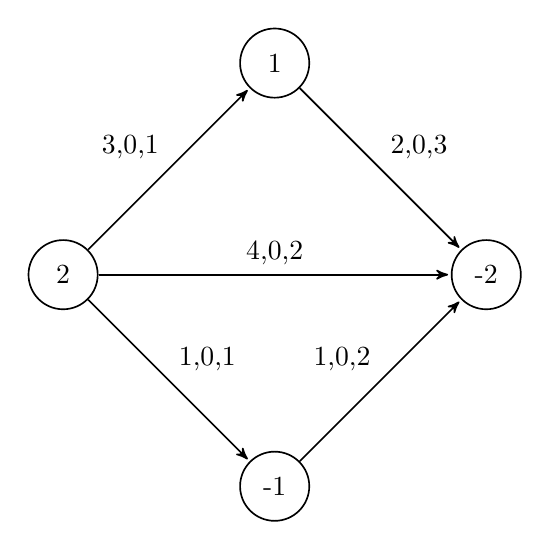
\begin{tikzpicture}[->,>=stealth',shorten >=1pt,auto,node distance=3.8cm,semithick]
        \node[state] (A) {2};
        \node[state] (B) [above right of=A] {1};
        \node[state] (C) [below right of=A] {-1};
        \node[state] (D) [below right of=B] {-2};

        \path (A) edge node {3,0,1} (B) % x_3
                  edge node {1,0,1} (C) % x_1
                  edge node {4,0,2} (D) % x_5
              (B) edge node {2,0,3} (D) % x_4
              (C) edge node {1,0,2} (D) % x_2
              ;
      \end{tikzpicture}
    \end{center}

    Now, we have a MCNF problem with all lower and upper bounds integer, and supplies
    and demands integer. So without loss of generality, this problem has an integer
    solution which is optimal.\\
\end{enumerate}
\end{document}
